\documentclass[11pt]{article}\usepackage[]{graphicx}\usepackage[]{color}
%% maxwidth is the original width if it is less than linewidth
%% otherwise use linewidth (to make sure the graphics do not exceed the margin)
\makeatletter
\def\maxwidth{ %
  \ifdim\Gin@nat@width>\linewidth
    \linewidth
  \else
    \Gin@nat@width
  \fi
}
\makeatother

\definecolor{fgcolor}{rgb}{0.345, 0.345, 0.345}
\newcommand{\hlnum}[1]{\textcolor[rgb]{0.686,0.059,0.569}{#1}}%
\newcommand{\hlstr}[1]{\textcolor[rgb]{0.192,0.494,0.8}{#1}}%
\newcommand{\hlcom}[1]{\textcolor[rgb]{0.678,0.584,0.686}{\textit{#1}}}%
\newcommand{\hlopt}[1]{\textcolor[rgb]{0,0,0}{#1}}%
\newcommand{\hlstd}[1]{\textcolor[rgb]{0.345,0.345,0.345}{#1}}%
\newcommand{\hlkwa}[1]{\textcolor[rgb]{0.161,0.373,0.58}{\textbf{#1}}}%
\newcommand{\hlkwb}[1]{\textcolor[rgb]{0.69,0.353,0.396}{#1}}%
\newcommand{\hlkwc}[1]{\textcolor[rgb]{0.333,0.667,0.333}{#1}}%
\newcommand{\hlkwd}[1]{\textcolor[rgb]{0.737,0.353,0.396}{\textbf{#1}}}%

\usepackage{framed}
\makeatletter
\newenvironment{kframe}{%
 \def\at@end@of@kframe{}%
 \ifinner\ifhmode%
  \def\at@end@of@kframe{\end{minipage}}%
  \begin{minipage}{\columnwidth}%
 \fi\fi%
 \def\FrameCommand##1{\hskip\@totalleftmargin \hskip-\fboxsep
 \colorbox{shadecolor}{##1}\hskip-\fboxsep
     % There is no \\@totalrightmargin, so:
     \hskip-\linewidth \hskip-\@totalleftmargin \hskip\columnwidth}%
 \MakeFramed {\advance\hsize-\width
   \@totalleftmargin\z@ \linewidth\hsize
   \@setminipage}}%
 {\par\unskip\endMakeFramed%
 \at@end@of@kframe}
\makeatother

\definecolor{shadecolor}{rgb}{.97, .97, .97}
\definecolor{messagecolor}{rgb}{0, 0, 0}
\definecolor{warningcolor}{rgb}{1, 0, 1}
\definecolor{errorcolor}{rgb}{1, 0, 0}
\newenvironment{knitrout}{}{} % an empty environment to be redefined in TeX

\usepackage{alltt}

\usepackage{fancyhdr}
\usepackage{amsmath}
\usepackage{float}
\usepackage[top=1in, bottom=1in, left=.5in, right=.5in]{geometry}
%\usepackage[font=small,labelfont=bf]{caption}

% Title.
% ------
\title{STAT 240 Homework 1}
\author{Rebecca Barter, Andrew Do and Kellie Ottoboni}
\IfFileExists{upquote.sty}{\usepackage{upquote}}{}
\begin{document}

\maketitle


 
 \section*{Question 1. Consider a box that contains 5 ``1'' tickets and 7 ``0'' tickets. Consider drawing 6 tickets from this box at random with replacement. Let $X_1, X_2, ..., X_6$ denote the 6 numbers you observe. Let $\bar{X}$ denote the average of the draws.}
 
 \subsection*{a) What is $E[\bar{X}]$?}
 \vspace{5mm}
 \noindent Recall that in class we showed that
 \begin{align*}
 E(\bar{X}) &= \bar{t}
 \end{align*}
 
 \noindent where $\bar{t}$ is the population mean. In particular, this implies that
 
\begin{align*}
E(\bar{X})= \frac{5}{12}
 \end{align*}
 
 
 \vspace{5mm}
 \subsection*{b) What is $SE[\bar{X}]$? (R hint: Be careful whether the function ``sd'' divides by the square root of $n$ or $n - 1$)}
  \vspace{5mm}
 \noindent Note that since this example corresponds to a simple box model with replacement, we have that
 $$SE(\bar{X}) = \sqrt{Var(\bar{X})} = \sqrt{\frac1n Var(t)}$$
 
 
 \noindent Using R and noting that the \texttt{sd()} function in R divides by $N-1$ rather than $N$, we found that (to 3dp)
 $$SE(\bar{X}) = 0.201$$
 

  \vspace{5mm}
 \subsection*{c) Use R to simulate 100,000 values of $\bar{X}$. Produce a histogram of these values. (R hint: Use the function sample).}
 
\begin{knitrout}
\definecolor{shadecolor}{rgb}{0.969, 0.969, 0.969}\color{fgcolor}\begin{figure}[H]

{\centering 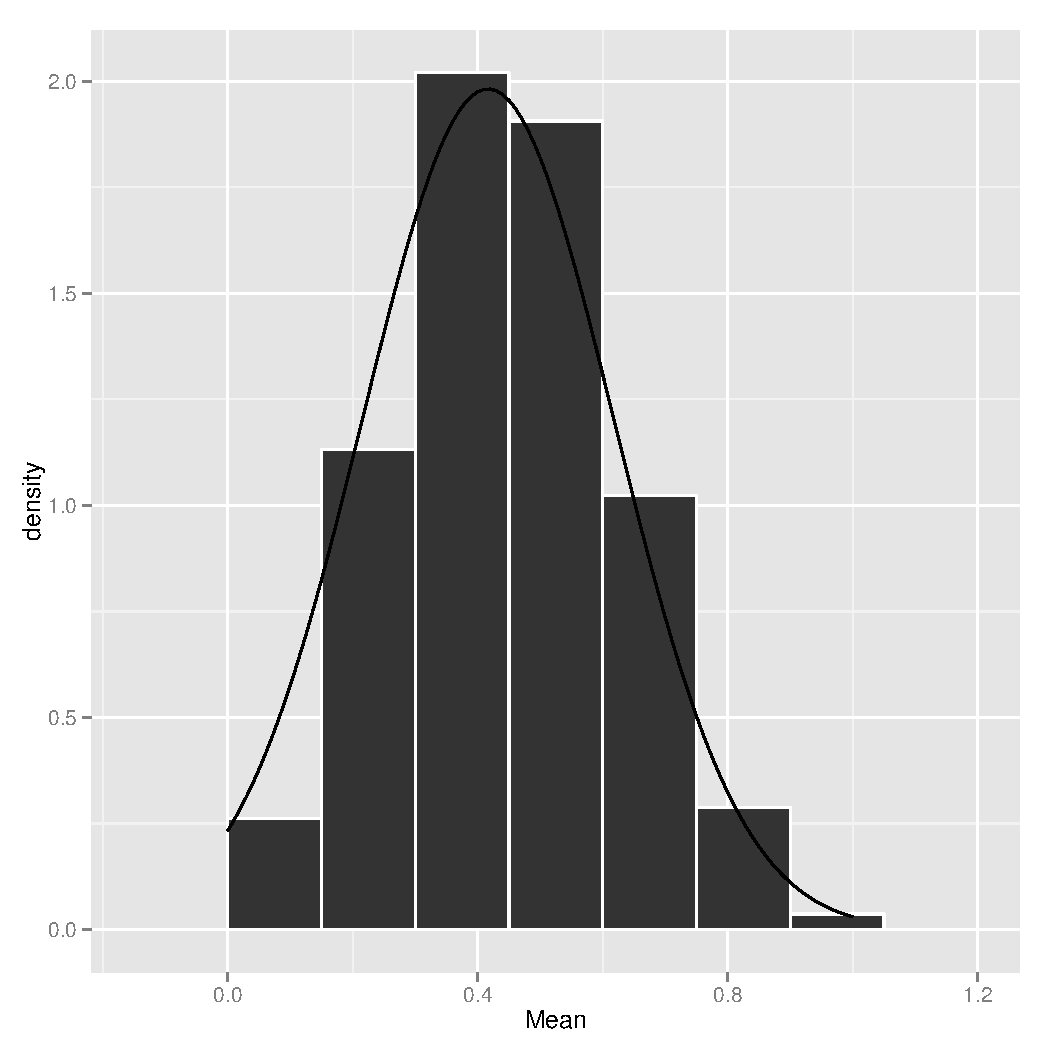
\includegraphics[width=\maxwidth]{figure/histogram_1c-1} 

}

\caption[Histogram of 100,000 simulated values of the sample mean when the sample was taken with replacement]{Histogram of 100,000 simulated values of the sample mean when the sample was taken with replacement}\label{fig:histogram_1c}
\end{figure}


\end{knitrout}
 
 \subsection*{d) Let $z_1 = E[\bar{X}] + SE[\bar{X}], ~ z_2 = E[\bar{X}] + 2 \times SE[\bar{X}]$, etc. For $z_1, ..., z_4$ calculate $P(\bar{X} > z_i)$ in three ways:
 \begin{itemize}
 \item Exactly, using the binomial distribution. (Hint: It will be easier to work with the sample sum than the sample average. R hint: Use function pbinom)
 \item Estimated using the values from part (c)
 \item Using the normal approximation. Use the continuity correction. (R hint: pnorm)
 \end{itemize}
 Do the same for $z_{-4},...,z_{-1}$ but calcualte $P(\bar{X} < z_i)$ instead of $P(\bar{X} > z_i)$. Make a table of your results and comment briefly}

% latex table generated in R 3.1.2 by xtable 1.7-4 package
% Fri Feb 13 11:01:37 2015
\begin{table}[H]
\centering
\begin{tabular}{|c|ccc|}
  \hline
z & Exact & EmpiricalEst & NormalApprox \\ 
  \hline
-4.00 & 0.00 & 0.00 & 0.00 \\ 
  -3.00 & 0.00 & 0.00 & 0.00 \\ 
  -2.00 & 0.04 & 0.04 & 0.06 \\ 
  -1.00 & 0.21 & 0.21 & 0.28 \\ 
  1.00 & 0.20 & 0.20 & 0.28 \\ 
  2.00 & 0.05 & 0.05 & 0.06 \\ 
  3.00 & 0.00 & 0.00 & 0.00 \\ 
  4.00 & 0.00 & 0.00 & 0.00 \\ 
   \hline
\end{tabular}
\caption{The exact value, empirical estimation and normal approximation of the probability.} 
\end{table}


\noindent We notice that the Empirical estimation using the results of our simulated value is extremely close the the exact value of the probabilities. On the other hand, the normal approximation is not nearly as accurate. This is likely because our sample size of 6 is very small and the asymptotic assumptions which underly the normal approximation are not yet accurate.



\subsection*{e) Repeat (a)-(d), this time sampling without replacement instead of with replacement. Use the hypergeometric distirbution instead fo the binomial distribuion (R hint: phyper)}


\noindent Note that since we are now sampling without replacement, we have that
$$E(\bar{X}) = \bar{t} = \frac{5}{12}$$

\noindent and
$$SE(\bar{X}) = \sqrt{Var(\bar{X})} = \sqrt{\frac{1}{n} Var(t) \left[\frac{N - n}{N - 1}\right]} = 0.149$$


\begin{knitrout}
\definecolor{shadecolor}{rgb}{0.969, 0.969, 0.969}\color{fgcolor}\begin{figure}[H]

{\centering 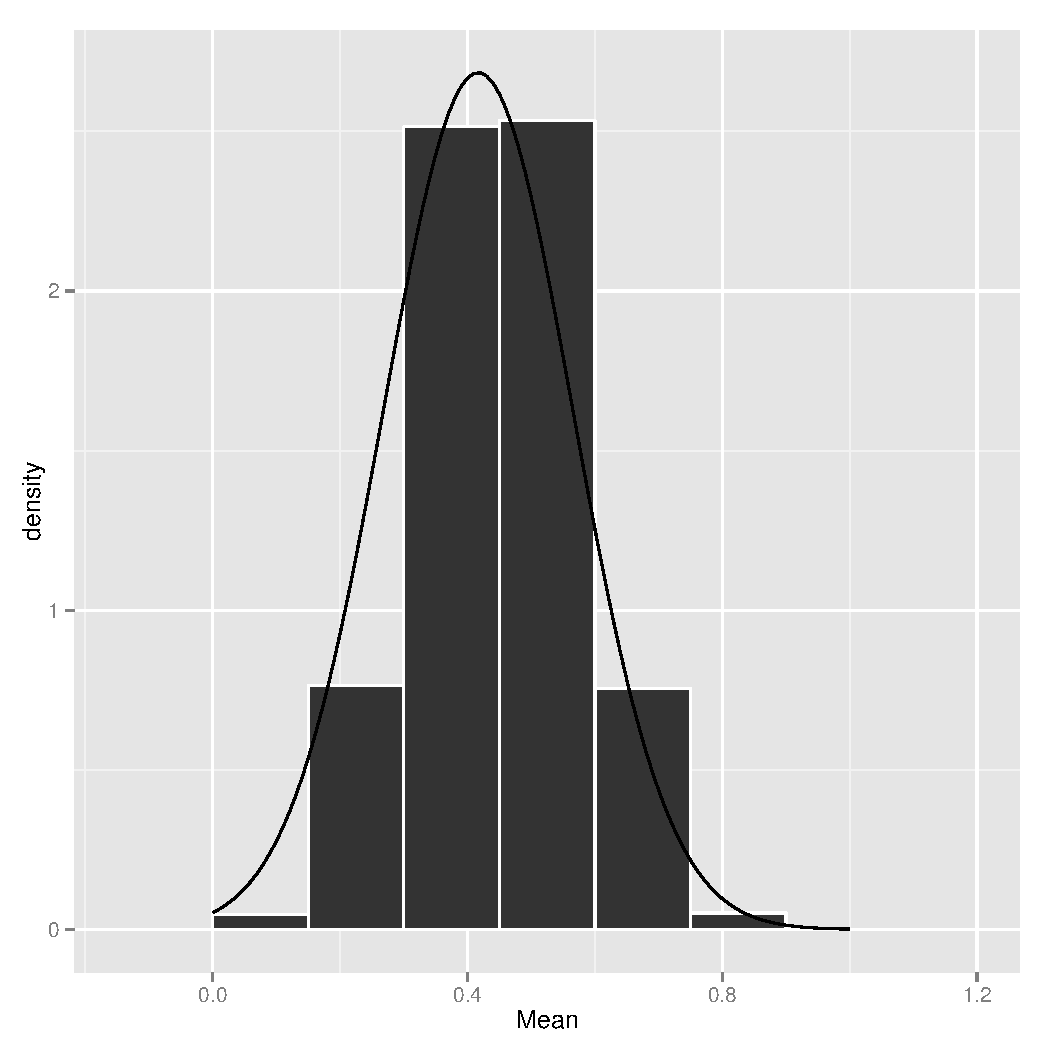
\includegraphics[width=\maxwidth]{figure/histogram_1e-1} 

}

\caption[Histogram of 100,000 simulated values of the sample mean when the sample was taken without replacement]{Histogram of 100,000 simulated values of the sample mean when the sample was taken without replacement}\label{fig:histogram_1e}
\end{figure}


\end{knitrout}

% latex table generated in R 3.1.2 by xtable 1.7-4 package
% Fri Feb 13 11:01:37 2015
\begin{table}[H]
\centering
\begin{tabular}{|c|ccc|}
  \hline
z & Exact & EmpiricalEst & NormalApprox \\ 
  \hline
-4.00 & 0.00 & 0.00 & 0.00 \\ 
  -3.00 & 0.00 & 0.00 & 0.01 \\ 
  -2.00 & 0.01 & 0.01 & 0.07 \\ 
  -1.00 & 0.12 & 0.12 & 0.33 \\ 
  1.00 & 0.12 & 0.12 & 0.33 \\ 
  2.00 & 0.01 & 0.01 & 0.07 \\ 
  3.00 & 0.00 & 0.00 & 0.01 \\ 
  4.00 & 0.00 & 0.00 & 0.00 \\ 
   \hline
\end{tabular}
\caption{The exact value, empirical estimation and normal approximation of the probability.} 
\end{table}


\end{document}
